\documentclass[12pt]{article}
\usepackage[a4paper,margin=0.75in]{geometry}
\usepackage[utf8]{inputenc}
\usepackage[OT1]{fontenc}
\usepackage[table,usenames,dvipsnames]{xcolor}
\usepackage{array}
\usepackage{varwidth}
\usepackage{tabularx}
\usepackage{amsmath}
\usepackage{hyperref}
\usepackage{enumitem}
\usepackage{graphicx}
\usepackage{tcolorbox}
\usepackage{multirow}
\usepackage{forest}
\usepackage{parskip}
\renewcommand*\familydefault{\sfdefault}

\newtcolorbox{mybox}[3][]
{
  colframe = #2!25,
  colback  = #2!10,
  coltitle = #2!20!black,  
  title    = {#3},
  #1,
}

\hypersetup{
    colorlinks=true,
    linkcolor=blue,
    filecolor=magenta,      
    urlcolor=cyan,
    pdftitle={Overleaf Example},
    pdfpagemode=FullScreen,
}

\title{\textbf{COL775 Assignment 1.1}\footnote{Models for this assignment can be found \href{https://drive.google.com/drive/folders/14zz1PKcDpUmSjqowXOoAwpHDdQYo3n3x?usp=sharing}{here}}}
\author{Aniruddha Deb \\ \texttt{2020CS10869}}
\date{March 2023}

\begin{document}

\maketitle

\section{Image Classification using ResNets}

The ResNet network was implemented in Pytorch and trained using SGD, with a 
learning rate of 0.1. For 100 epochs, we used a stepped learning rate schedule,
which multiplies the learning rate by 0.1 every 20 epochs.

\begin{figure}[!htbp]
    \centering
    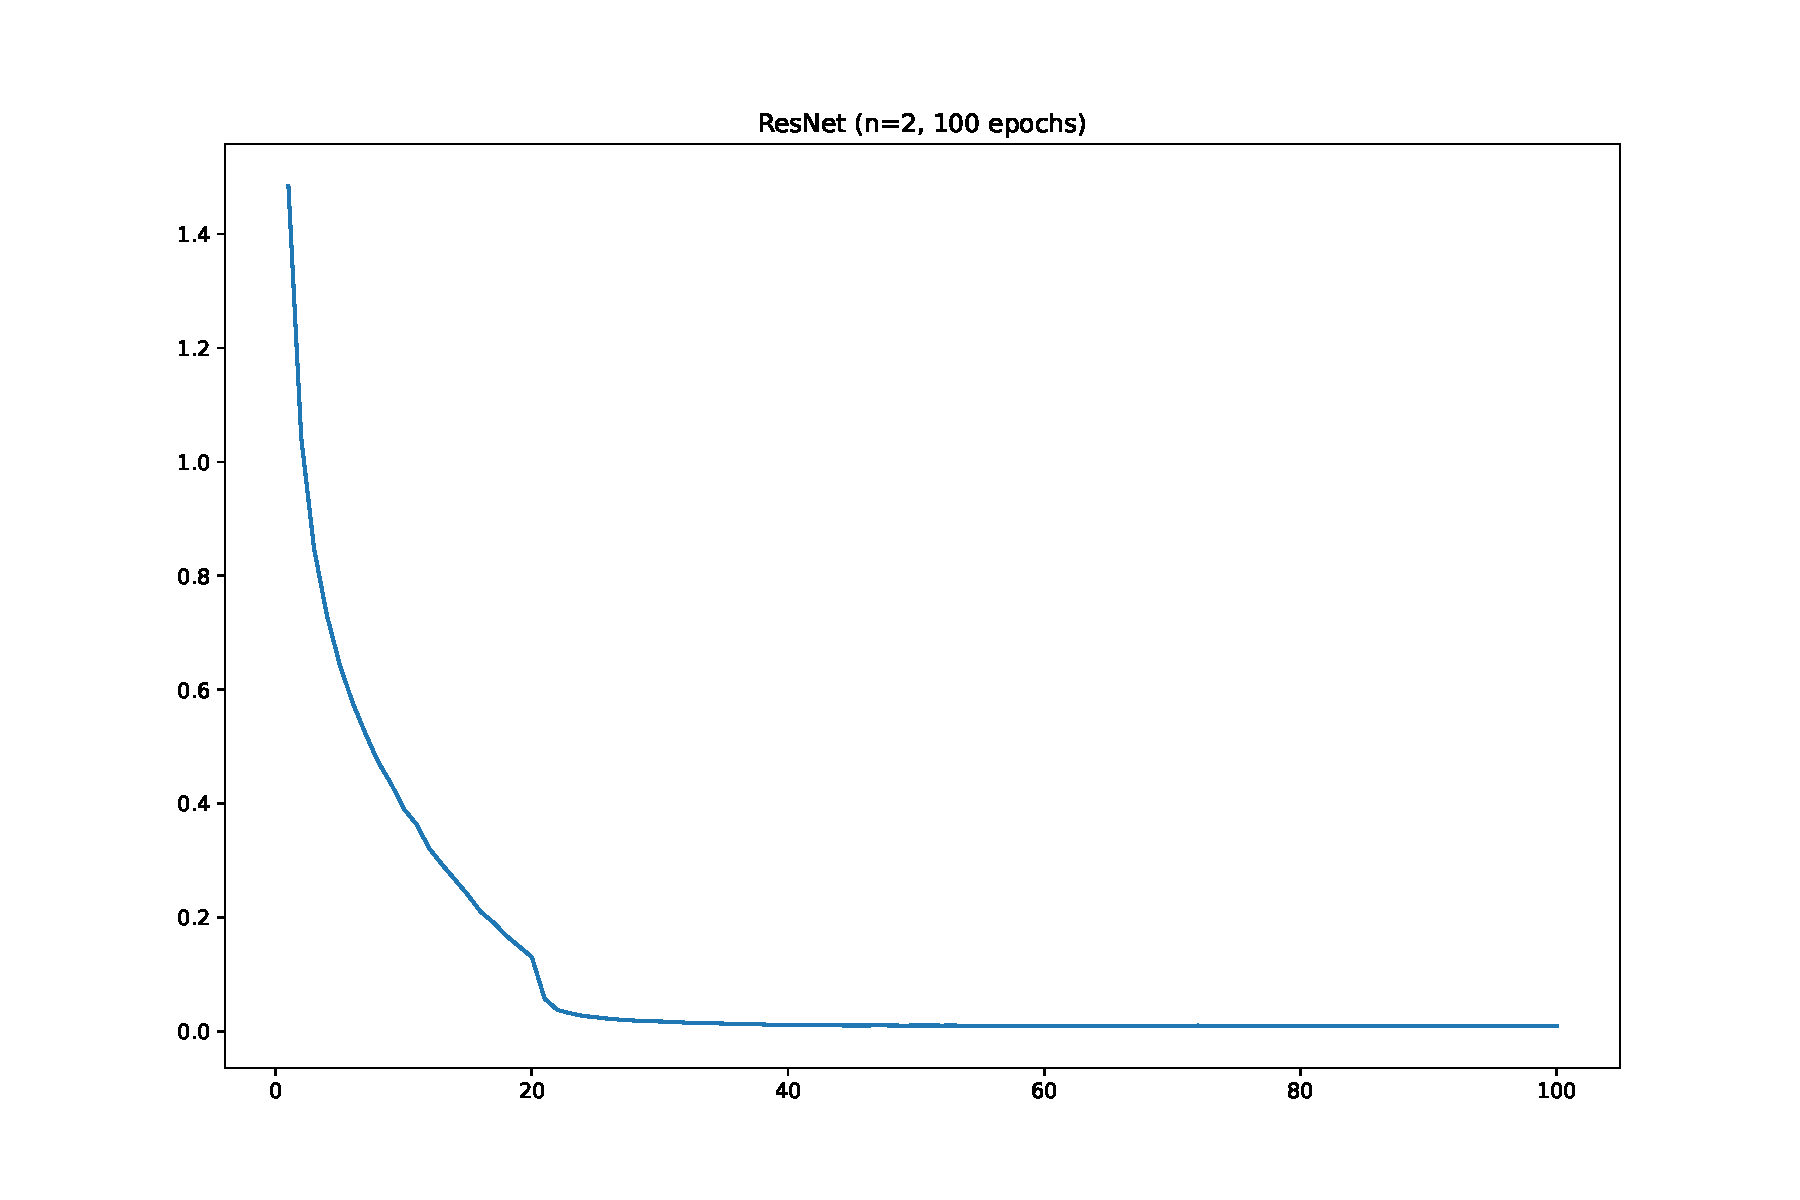
\includegraphics[width=0.7\textwidth]{q1_part2.pdf}
\end{figure}

With validation and early stopping, we used a more aggressive learning rate
schedule, as we noticed the validation loss being very unstable with a high
learning rate, which impacted the patience and led it to prematurely early 
stop. We reduced the step size to 5 and increased the multiplier to 0.2.

\begin{figure}[!htbp]
    \centering
    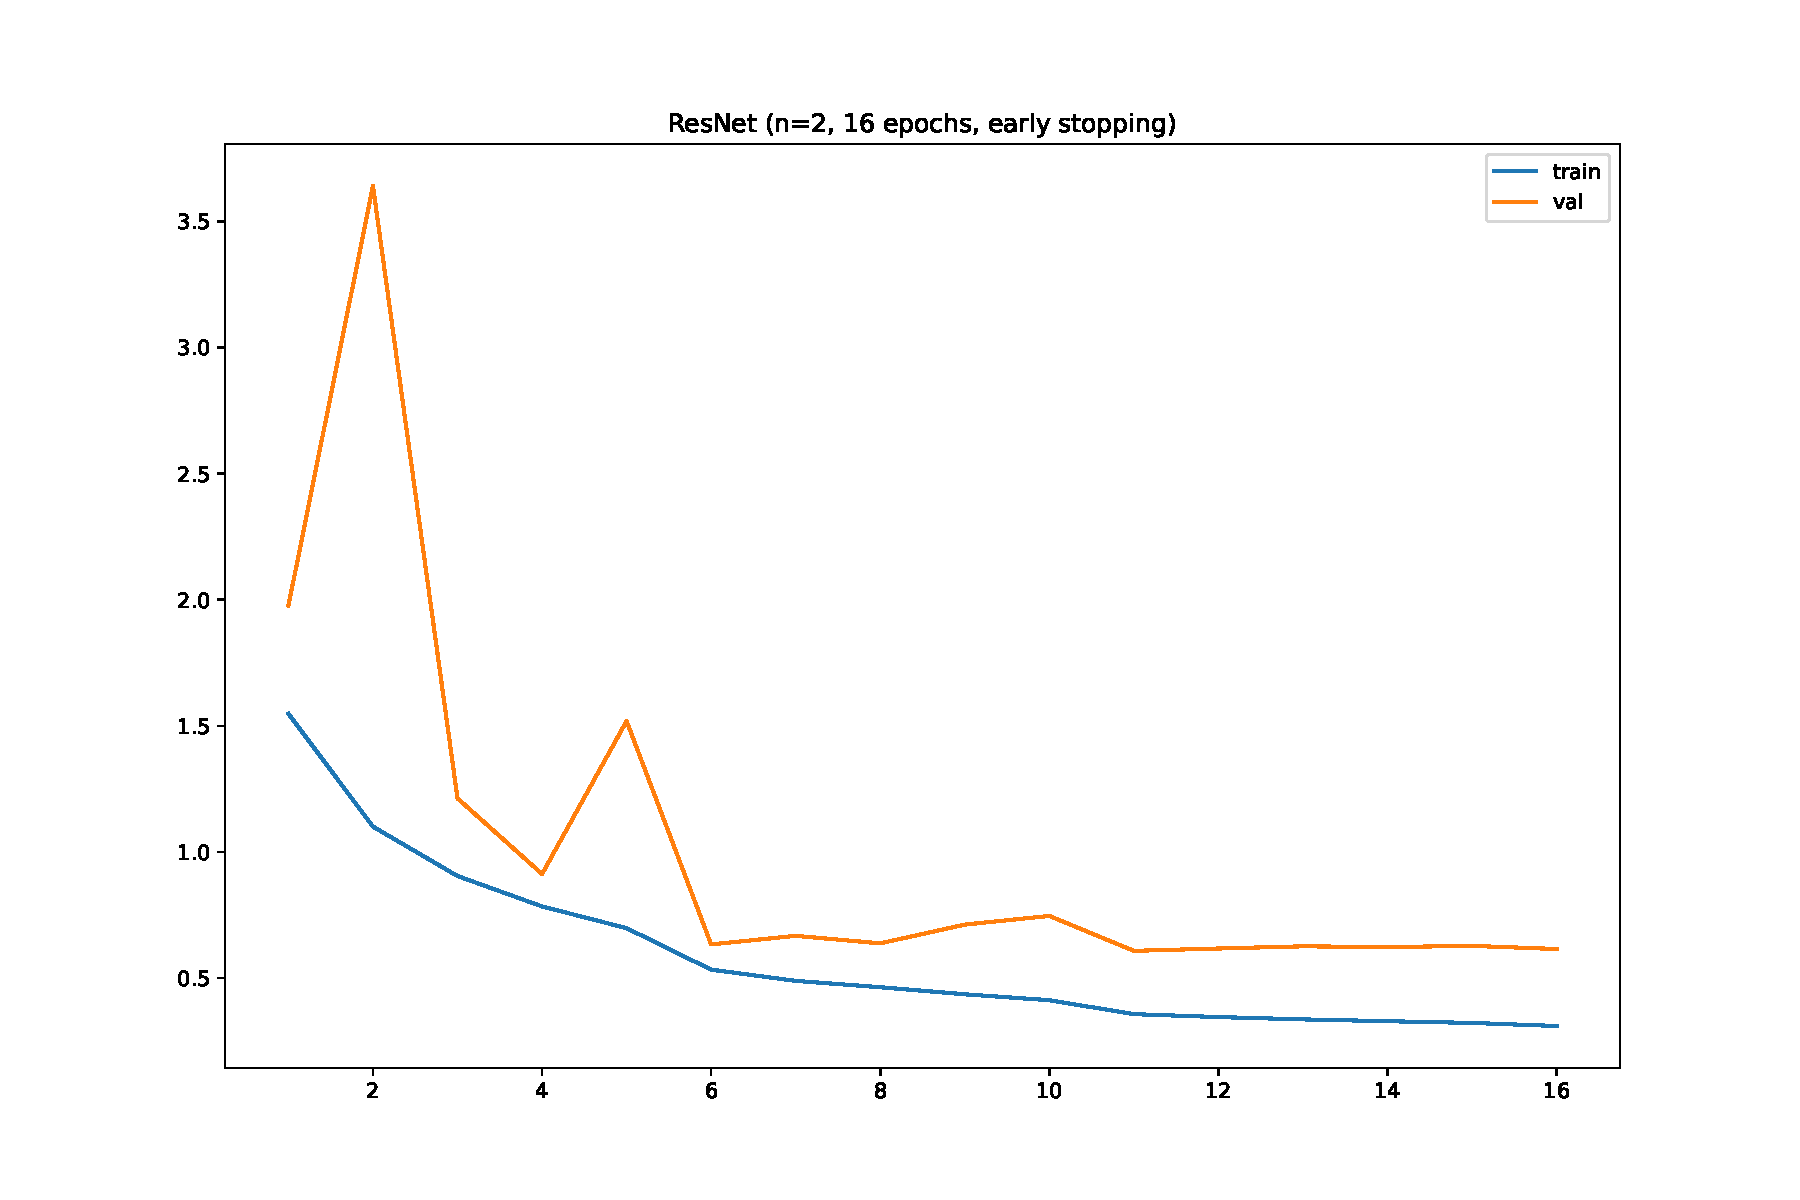
\includegraphics[width=0.7\textwidth]{q1_part3.pdf}
\end{figure}

The final statistics are as follows:

\begin{center}
\begin{tabular}{|l|c|c|c|}
    \hline
    & Accuracy & F1 micro & F1 macro \\ 
    \hline
    train & 0.916 & 0.916 & 0.916 \\
    val & 0.797 & 0.797 & 0.796 \\
    test & 0.791 & 0.791 & 0.790 \\
    \hline
\end{tabular}
\end{center}

\section{Impact of Normalization}

\subsection{Implementation Details}
Normalization was implemented by taking inspiration from the PyTorch
implementation, which uses a base Normalization class, and subclasses which
use it's buffers. The weight buffers are used by all the implementations, and 
BatchNorm and InstanceNorm would use the mean/stdev buffers if needed. Layer
normalization does not make use of any buffers, and neither does group 
normalization.

\begin{center}
\begin{figure}[!htbp]
    \centering
    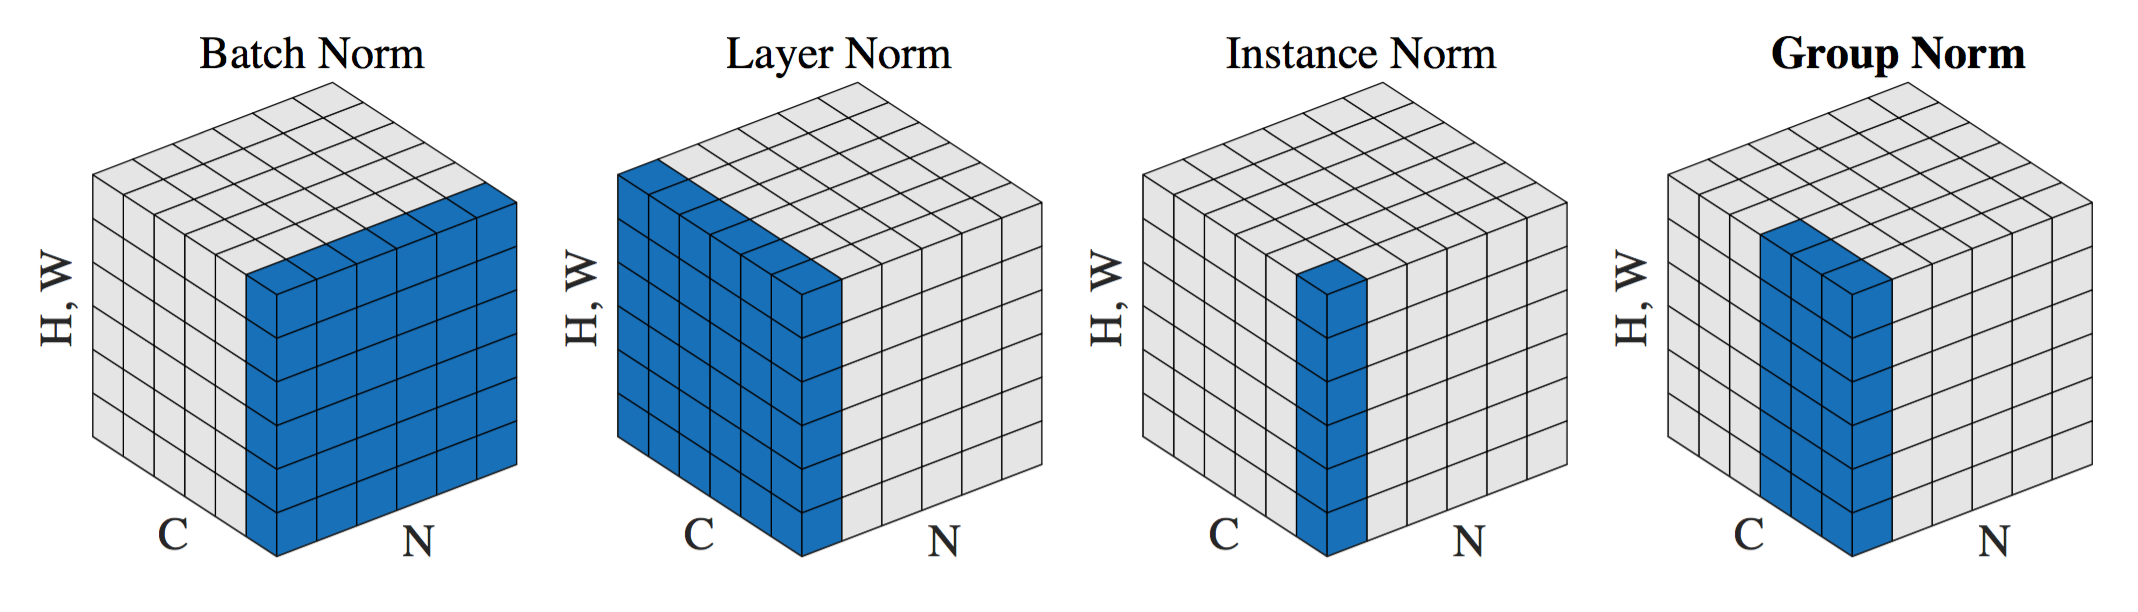
\includegraphics[width=0.9\textwidth]{norm_types.png}
    \caption{Normalization schemes (Taken from He et al)}
\end{figure}
\end{center}

A minor implementation detail was clipping the rho parameter in BatchInstanceNorm:
the \href{https://github.com/hyeonseobnam/Batch-Instance-Normalization/blob/master/main.py#L226}{original implementation} 
did this while training, and we do the same. We use 16 groups in the Group 
Normalizer implementation (down from the original 32 suggested in the original
paper) because of the fewer number of layers in our ResNet implementation.
Another constraint of our GroupNorm implementation is that the number of groups
always has to be a multiple of the number of channels.

\pagebreak 
\subsection{Results}
The training results and loss curves of the various normalization schemes are
shown on the next page. All schemes were trained using early stopping with the
same learning rate/scheduler as before, to be comparable to the default PyTorch 
implementation. BatchNorm constantly outperforms the other normalization
schemes, and BatchInstanceNorm would probably be setting all it's gates to 1,
to use the BatchNorm layers more.

\begin{center}
\begin{tabular}{|l|r|c|c|c|}
    \hline
    Norm & set & Accuracy & F1 micro & F1 macro \\
    \hline
    \multirow{3}{*}{BN (torch)}%
    & train & 0.913 & 0.913 & 0.913 \\
    & val & \textbf{0.791} & \textbf{0.791} & \textbf{0.790} \\
    & test & 0.783 & 0.783 & 0.783 \\
    \hline

    \hline
    \multirow{3}{*}{BN}%
    & train & 0.913 & 0.913 & 0.913 \\
    & val & 0.782 & 0.782 & 0.781 \\
    & test & \textbf{0.785} & \textbf{0.785} & \textbf{0.785} \\
    \hline

    \hline
    \multirow{3}{*}{IN}%
    & train & 0.725 & 0.725 & 0.724 \\
    & val & 0.684 & 0.684 & 0.682 \\
    & test & 0.669 & 0.669 & 0.667 \\
    \hline

    \hline
    \multirow{3}{*}{BIN}%
    & train & \textbf{0.933} & \textbf{0.933} & \textbf{0.932} \\
    & val & 0.788 & 0.788 & 0.787 \\
    & test & 0.780 & 0.780 & 0.780 \\
    \hline

    \hline
    \multirow{3}{*}{LN}%
    & train & 0.766 & 0.766 & 0.765 \\
    & val & 0.725 & 0.725 & 0.723 \\
    & test & 0.727 & 0.727 & 0.725 \\
    \hline

    \hline
    \multirow{3}{*}{GN}%
    & train & 0.757 & 0.757 & 0.756 \\
    & val & 0.706 & 0.706 & 0.705 \\
    & test & 0.699 & 0.699 & 0.697 \\
    \hline

    \hline
    \multirow{3}{*}{NN}%
    & train & 0.737 & 0.737 & 0.736 \\
    & val & 0.714 & 0.714 & 0.712 \\
    & test & 0.706 & 0.706 & 0.705 \\
    \hline
\end{tabular}
\end{center}

\begin{center}
\begin{figure}[!htbp]
    \centering
    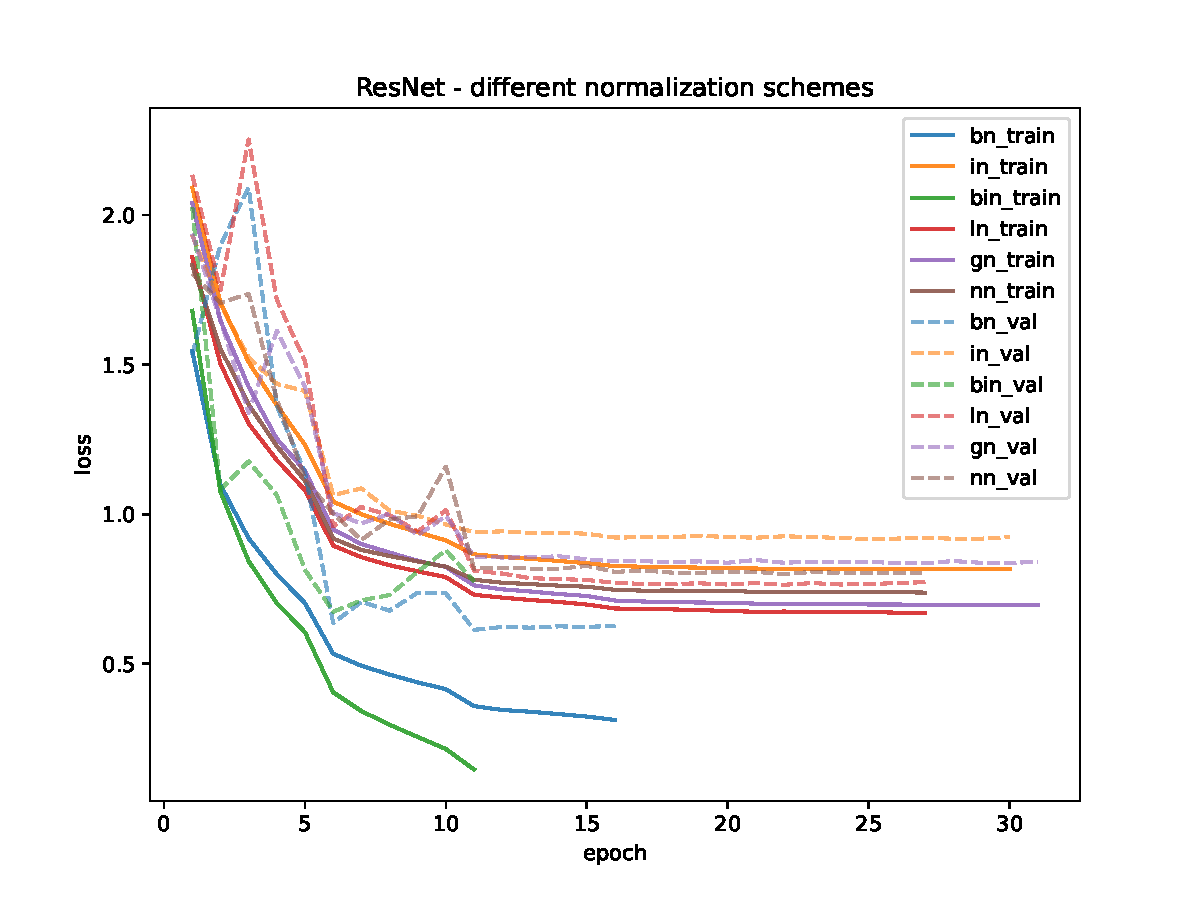
\includegraphics[width=0.7\textwidth]{q2_part3.pdf}
\end{figure}
\end{center}

\pagebreak

\subsection{BatchNorm vs GroupNorm}

We find results contrary to those mentioned by Wu and He: BatchNorm outperforms
GroupNorm in our setting. Both reach the same training accuracy, but GroupNorm
falls short on the validation accuracy compared to BatchNorm. This may also be 
attributed to the fact that our model simply has fewer filters (64 at max), 
while the original ResNet had a minimum of 64 and a maximum of 512 filters, and
was much deeper, hence the benefits of GroupNorm are not apparent.

\begin{center}
\begin{figure}[!htbp]
    \centering
    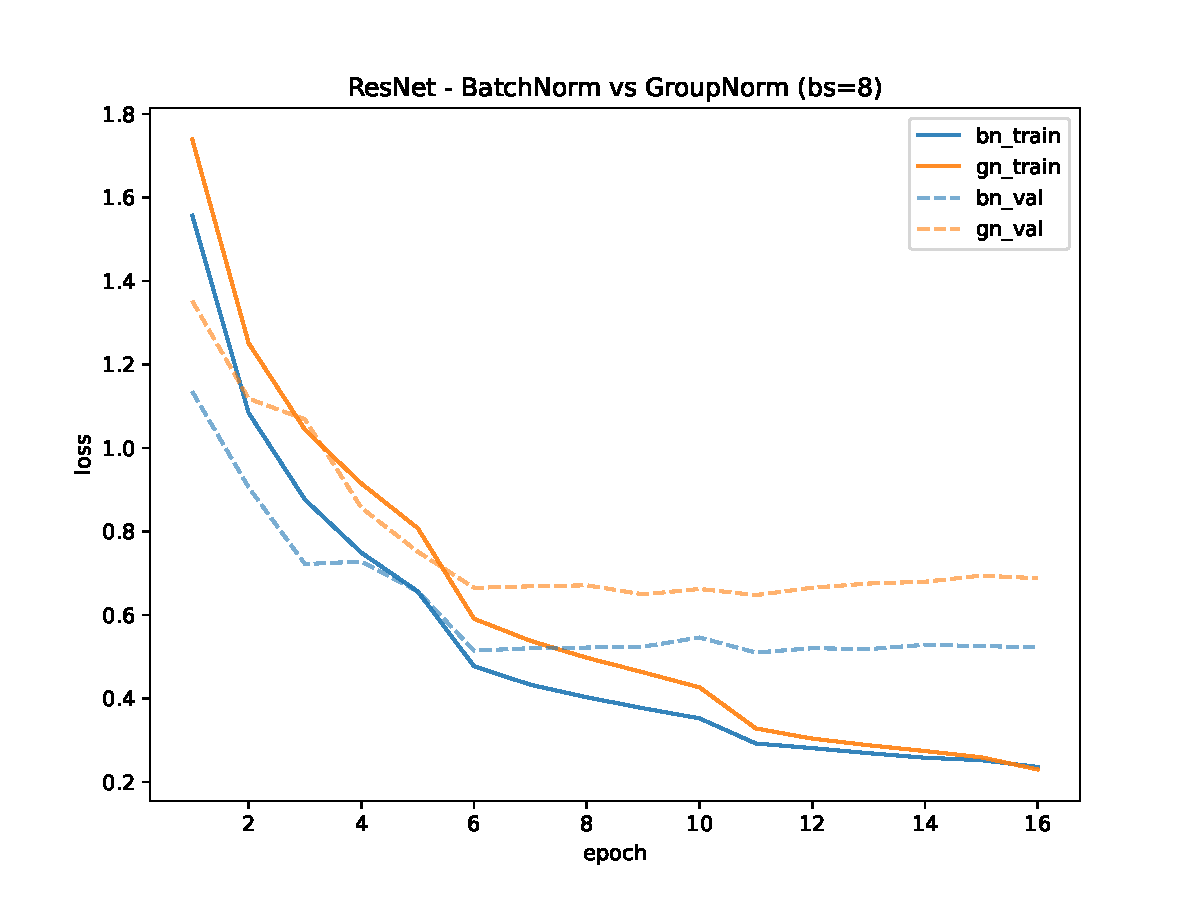
\includegraphics[width=0.7\textwidth]{q2_part6.pdf}
\end{figure}
\end{center}

The comparision with batches of size 128 is as follows:

\begin{center}
\begin{tabular}{|l|r|c|c|c|}
    \hline
    Norm & set & Accuracy & F1 micro & F1 macro \\
    \hline
    \multirow{3}{*}{BN-128}%
    & train & 0.913 & 0.913 & 0.913 \\
    & val & 0.791 & 0.791 & 0.790 \\
    & test & 0.783 & 0.783 & 0.783 \\
    \hline

    \multirow{3}{*}{GN-128}%
    & train & 0.757 & 0.757 & 0.756 \\
    & val & 0.706 & 0.706 & 0.705 \\
    & test & 0.699 & 0.699 & 0.697 \\
    \hline

    \hline
    \multirow{3}{*}{BN-8}%
    & train & \textbf{0.956} & \textbf{0.956} & \textbf{0.956} \\
    & val & \textbf{0.828} & \textbf{0.828} & \textbf{0.828} \\
    & test & \textbf{0.818} & \textbf{0.818} & \textbf{0.818} \\
    \hline

    \hline
    \multirow{3}{*}{GN-8}%
    & train & 0.939 & 0.939 & 0.939 \\
    & val & 0.789 & 0.789 & 0.788 \\
    & test & 0.784 & 0.784 & 0.783 \\
    \hline
\end{tabular}
\end{center}

Noticeably, the models with smaller batch sizes perform better than the ones 
with larger batch sizes. According to Goodfellow, this is because smaller 
batch sizes have a regularizing effect: the path the optimizer takes through
the loss landscape is noisier, and as a result it has more chance of falling 
into a local minima (as there are several equally good local minima, and more
saddle points than local minima in a high-dimensional space).

\pagebreak
\subsection{Quantile Plot}

The quantile plot of the first validation example is plotted below: the features
are expressed as a 64-dimensional vector. We sort this vector and plot the first,
twentieth, eightieth and ninety-ninth quantile of features. 

\begin{center}
\begin{figure}[!htbp]
    \centering
    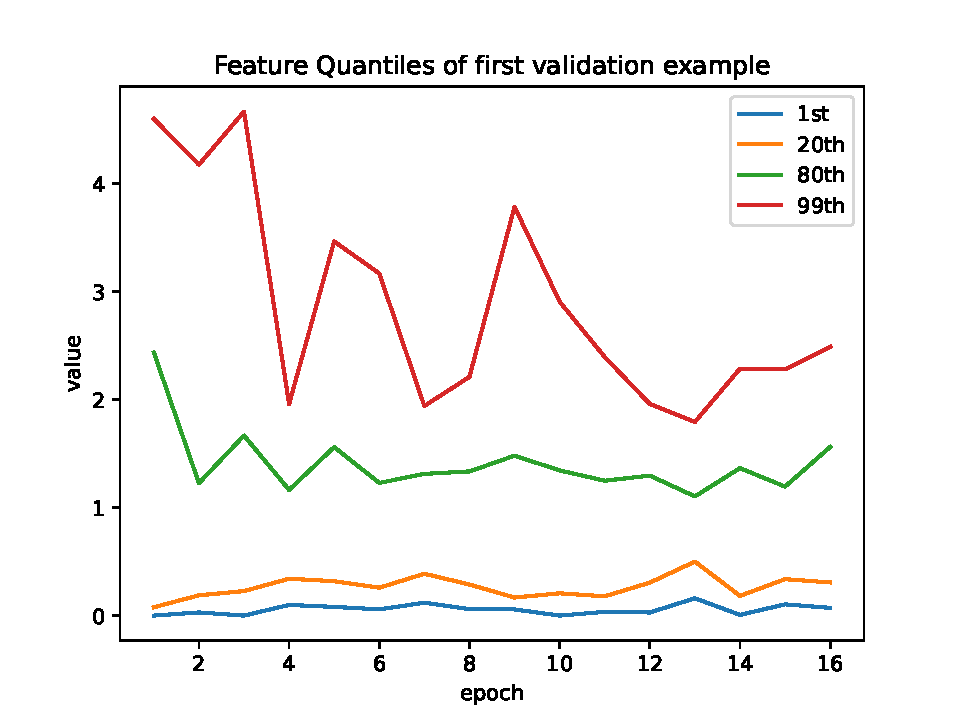
\includegraphics[width=0.7\textwidth]{q2_part7.pdf}
\end{figure}
\end{center}

Although it is noisy, we see that the upper quantiles decrease, while the 
lower quantiles marginally increase for the best-trained model (which is around
epochs 10-13). This shows that the features converge to the mean as the model
trains.

\end{document}
